\newcommand{\trivialSigmaAlgebra}{
    \begin{example}{\texorpdfstring{$\sigma$}{sigma}-álgebra Trivial}{trivial_sigma_algebra}
        Seja $X$ um conjunto. Então $\Sigma=\{\varnothing, X\}$ é uma \nameref{def:sigma_algebra} conhecida como a \textbf{\texorpdfstring{$\sigma$}{sigma}-álgebra trivial de $X$}.
    \end{example}
}

\newcommand{\powerSetSigmaAlgebra}{
    \begin{example}{\texorpdfstring{$\sigma$}{sigma}-álgebra das Partes}{power_set_sigma_algebra}
        Seja $X$ um conjunto. Então $\Sigma=\powerset{X}$ é uma \nameref{def:sigma_algebra} conhecida como a \textbf{\texorpdfstring{$\sigma$}{sigma}-álgebra das partes de $X$}.
    \end{example}
}

\newcommand{\countableSetsSigmaAlgebra}{
    \begin{example}{\texorpdfstring{$\sigma$}{sigma}-álgebra dos Conjuntos Enumeráveis}{countable_sets_sigma_algebra}
        Seja $X$ um conjunto não enumerável. Então
        \begin{equation*}
            \Sigma=\{E\in X; \ E\text{ é enumerável ou } \complement(E) \text{ é enumerável}\}
        \end{equation*}
        é uma \nameref{def:sigma_algebra} conhecida como a \textbf{\texorpdfstring{$\sigma$}{sigma}-álgebra dos conjuntos enumeráveis e co-enumeráveis de $X$}.
    \end{example}
}

\newcommand{\countingMeasure}{
    \begin{example}{Medida de Contagem}{counting_measure}
        Seja $(X,\Sigma)$ um \nameref{def:measure_space} onde $X$ é um conjunto não enumerável e $\Sigma$ é a \nameref{exm:countable_sets_sigma_algebra}. A função
    \begin{equation*}
        \mu (E)=
        \begin{cases}
            \#E, \text{ se } E \text{ é finito}, \\
            +\infty, \text{ se } E \text{ é infinito},
        \end{cases}
    \end{equation*}
    é uma medida em $X$.
    \end{example}
}

\newcommand{\diracMeasure}{
    \begin{example}{Medida de Dirac}{dirac_measure}
        Sejam $(X,\powerset{X})$ um \nameref{def:measure_space} e $x_0\in X$ um ponto fixado. A função
    \begin{equation*}
        \mu (E)=
        \begin{cases}
            1, \text{ se } x_0\in E, \\
            0, \text{ se } x_0\not\in E,
        \end{cases}
    \end{equation*}
    é uma medida em $X$.
    \end{example}
}

\newcommand{\constantFunction}{
    \begin{example}{Função Constante}{constant_function}
        Seja $(X,\Sigma)$ um espaço mensurável e $f:(X,\Sigma)\rightarrow (\R,\mathcal{B})$ uma função constante. Então $f$ é uma função mensurável.
    \end{example}
}

\newcommand{\characteristicFunction}{
    \begin{example}{Função Característica}{characteristic_function}
        Seja $(X,\Sigma)$ um espaço mensurável, $E\in \Sigma$ um conjunto mensurável e $\chi_{E}:(X,\Sigma)\rightarrow (\R,\mathcal{B})$ uma função definida por:
    \begin{equation*}
        \chi_{E}(x)=
        \begin{cases}
            1, x\in E \\
            0, x\in \complement(E)
        \end{cases}.
    \end{equation*}
    \end{example}
}

\newcommand{\counterExampleUniformConvergence}{
    \begin{example}{Convergência Uniforme \texorpdfstring{$\not\Rightarrow$}{->} Convergência em $L_p$}{counter_example_uniform_convergence}
        Seja $$f_n:x\in X\mapsto n^{-1}\chi_{(0,n)}\in\R$$ para todo $n\in\N$. Esta sequência converge uniformemente para $0$ pois, para todo $\varepsilon>0$ existe, pelo princípio de arquimedes, $N(\varepsilon) \in \N$ tal que $0<N^{-1}<\varepsilon$. Se $n\geq N$, então $n^{-1}<\varepsilon$. Por fim, note que , para todo $x\in X$, $f_n(x)\leq n^{-1}<\varepsilon$, o que mostra a converência uniforme. No entanto, $\norm{f_n}_p=1$, logo $\lim \norm{f_n-0}_p \neq 0$ e $f_n$ não pode convergir para $0$ em $L_p$.
    \end{example}
}

\newcommand{\counterExamplePointwiseConvergence}{
    \begin{example}{Convergência Pontual \texorpdfstring{$\not\Rightarrow$}{->} Convergência em $L_p$}{counter_example_pointwise_convergence}
        Seja $$f_n:x\in X\mapsto \chi_{(n,n+1)}\in\R$$ para todo $n\in\N$. Esta sequência converge pontualmente para $0$ pois, fixado um $x\in X$, $f_n(x)= 0$ para todo $n > x$, o que mostra a converência de $(f_n(x))$. No entanto, $\norm{f_n}_p=1$, logo $\lim \norm{f_n-0}_p \neq 0$ e $f_n$ não pode convergir para $0$ em $L_p$.
    \end{example}
}

\newcommand{\counterExampleAEConvergence}{
    \begin{example}{Convergência \texorpdfstring{$\mu$}{u}-qtp \texorpdfstring{$\not\Rightarrow$}{->} Convergência em $L_p$}{counter_example_ae_convergence}
        Seja $$f_n:x\in X\mapsto n\chi_{(0,\frac{1}{n})}\in\R$$ para todo $n\in\N$. Esta sequência converge pontualmente para $0$ exceto no ponto $\{0\}$, que tem medida nula, o que conclui a converência $\mu$-qtp. No entanto, $\norm{f_n}_p=1$, logo $\lim \norm{f_n-0}_p \neq 0$ e $f_n$ não pode convergir para $0$ em $L_p$.
    \end{example}
}

\newcommand{\counterExampleLpConvergence}{
    \begin{example}{Convergência em $L_p$ \texorpdfstring{$\not\Rightarrow$}{->} Convergência \texorpdfstring{$\mu$}{u}-qtp}{counter_example_lp_convergence}
        Seja $$f_n:x\in X\mapsto \chi_{\left(\frac{j}{2^k}, \frac{(j+1)}{2^k}\right)}\in\R$$ para todo $k\in\N$ e $n=2^k+j$ com $0\leq j < 2^k$.
        
        Visualize essa sequência como ondas quadradas de período progressivamente menores, percorrendo o intervalo entre $0$ e $1$.


        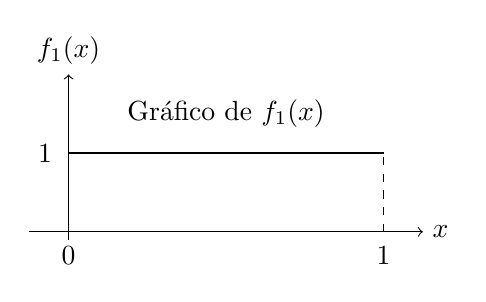
\begin{tikzpicture}
    % Draw x and y axes
    \draw[->] (-0.5, 0) -- (4.5, 0) node[right] {$x$};
    \draw[->] (0, -0.1) -- (0, 2) node[above] {$f_1(x)$};
    
    % Draw the function f_1
    \draw[thick] (0, 1) -- (4, 1); % f_1 is 1 in [0,1]
    %\draw[dashed] (0, 0) -- (4, 0); % Dashed line at y = 0
    
    % Vertical lines to close the graph at 0 and 1
    %\draw[thick] (0, 0) -- (0, 1);
    \draw[dashed] (4, 0) -- (4, 1);
    
    % Labels for the intervals and function values
    \node at (4,-0.3) {$1$};
    \node at (0,-0.3) {$0$};
    \node at (-0.3,1) {$1$};

    % Add title
    \node at (2, 1.5) {Gráfico de $f_1(x)$};
    
\end{tikzpicture}

\begin{minipage}{0.45\textwidth}
    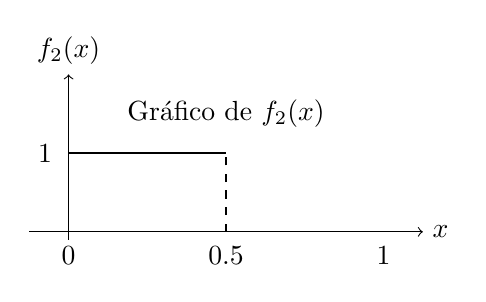
\begin{tikzpicture}
        % Draw x and y axes
        \draw[->] (-0.5, 0) -- (4.5, 0) node[right] {$x$};
        \draw[->] (0, -0.1) -- (0, 2) node[above] {$f_2(x)$};
        
        % Draw the function f_2
        \draw[thick] (0, 1) -- (2, 1); % f_2 is 1 in [0,0.5]
        \draw[dashed] (2, 0) -- (2, 1);
        
        % Labels for the intervals and function values
        \node at (4,-0.3) {$1$};
        \node at (2,-0.3) {$0.5$};
        \node at (0,-0.3) {$0$};
        \node at (-0.3,1) {$1$};
    
        % Add title
        \node at (2, 1.5) {Gráfico de $f_2(x)$};
    \end{tikzpicture}
\end{minipage}
\begin{minipage}{0.45\textwidth}
    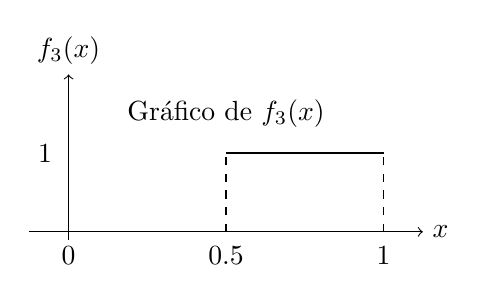
\begin{tikzpicture}
        % Draw x and y axes
        \draw[->] (-0.5, 0) -- (4.5, 0) node[right] {$x$};
        \draw[->] (0, -0.1) -- (0, 2) node[above] {$f_3(x)$};
        
        % Draw the function f_3
        \draw[thick] (2, 1) -- (4, 1); % f_3 is 1 in [0.5,1]
        \draw[dashed] (4, 0) -- (4, 1);
        \draw[dashed] (2, 0) -- (2, 1);
        
        % Labels for the intervals and function values
        \node at (4,-0.3) {$1$};
        \node at (2,-0.3) {$0.5$};
        \node at (0,-0.3) {$0$};
        \node at (-0.3,1) {$1$};
    
        % Add title
        \node at (2, 1.5) {Gráfico de $f_3(x)$};
    \end{tikzpicture}
\end{minipage}

\begin{minipage}{0.24\textwidth}
    \begin{tikzpicture}
        % Draw x and y axes
        \draw[->] (-0.25, 0) -- (2.25, 0) node[right] {$x$};
        \draw[->] (0, -0.1) -- (0, 2) node[above] {$f_4(x)$};
        
        % Draw the function f_4
        \draw[thick] (0, 1) -- (0.5, 1); % f_4 is 1 in [0,0.25]
        \draw[dashed] (0.5, 0) -- (0.5, 1);
        
        % Labels for the intervals and function values
        \node at (2,-0.3) {$1$};
        \node at (0,-0.3) {$0$};
        \node at (-0.3,1) {$1$};
    \end{tikzpicture}
\end{minipage}
\begin{minipage}{0.24\textwidth}
    \begin{tikzpicture}
        % Draw x and y axes
        \draw[->] (-0.25, 0) -- (2.25, 0) node[right] {$x$};
        \draw[->] (0, -0.1) -- (0, 2) node[above] {$f_5(x)$};
        
        % Draw the function f_5
        \draw[thick] (0.5, 1) -- (1, 1); % f_5 is 1 in [0.25,0.5]
        \draw[dashed] (0.5, 0) -- (0.5, 1);
        \draw[dashed] (1, 0) -- (1, 1);
        
        % Labels for the intervals and function values
        \node at (2,-0.3) {$1$};
        \node at (0,-0.3) {$0$};
        \node at (-0.3,1) {$1$};
    \end{tikzpicture}
\end{minipage}
\begin{minipage}{0.24\textwidth}
    \begin{tikzpicture}
        % Draw x and y axes
        \draw[->] (-0.25, 0) -- (2.25, 0) node[right] {$x$};
        \draw[->] (0, -0.1) -- (0, 2) node[above] {$f_6(x)$};
        
        % Draw the function f_6
        \draw[thick] (1, 1) -- (1.5, 1); % f_6 is 1 in [0.5,0.75]
        \draw[dashed] (1, 0) -- (1, 1);
        \draw[dashed] (1.5, 0) -- (1.5, 1);
        
        % Labels for the intervals and function values
        \node at (2,-0.3) {$1$};
        \node at (0,-0.3) {$0$};
        \node at (-0.3,1) {$1$};
    \end{tikzpicture}
\end{minipage}
\begin{minipage}{0.24\textwidth}
    \begin{tikzpicture}
        % Draw x and y axes
        \draw[->] (-0.25, 0) -- (2.25, 0) node[right] {$x$};
        \draw[->] (0, -0.1) -- (0, 2) node[above] {$f_7(x)$};
        
        % Draw the function f_7
        \draw[thick] (1.5, 1) -- (2, 1); % f_7 is 1 in [0.75,1]
        \draw[dashed] (1.5, 0) -- (1.5, 1);
        \draw[dashed] (2, 0) -- (2, 1);
        
        % Labels for the intervals and function values
        \node at (2,-0.3) {$1$};
        \node at (0,-0.3) {$0$};
        \node at (-0.3,1) {$1$};
    \end{tikzpicture}
\end{minipage}
        
        Esta sequência converge pontualmente para $0$ em $L_1$ pois
        
        \begin{equation*}
            \lim_{n\rightarrow \infty} \norm{f_n-0}_1 = \lim_{n\rightarrow \infty} \int_{X} \abs{f_n(x)-0} d\mu =  \lim_{n\rightarrow \infty} \int_{\frac{j}{2^k}}^{\frac{j+1}{2^k}} 1 d\mu = \lim_{n\rightarrow \infty} 2^k = 0.
        \end{equation*}
        
        No entanto, $(f_n)$ não converge $\mu$-qtp (logo, nem pontualmente, nem uniformemente).
    \end{example}
}